\begin{frame}{embeddings as teachers}{introduction}
    \begin{itemize}
        \item   \textbf{question}:
            \begin{itemize}
                \item   how can we provide extra training information without additional data labels 
            \end{itemize}
        \bigskip
        \item   \textbf{idea}: 
            \begin{itemize}
                \item use proven pre-trained embeddings (e.g., VGGish, OpenL3, \ldots)
            \end{itemize}
        \bigskip
        \item<2->   \textbf{goals}:
            \begin{itemize}
                \item   \textit{impart knowledge} of pre-trained deep models 
                \item   \textit{improve model generalization} by utilizing pre-trained embeddings
                \item   \textit{reduce model complexity}
            \end{itemize}
				\bigskip
				\item<3-> \textbf{general approach}:
					\begin{itemize}
						\item  combine transfer learning and knowledge distillation ideas
					\end{itemize}
    \end{itemize}
\end{frame}

\begin{frame}{embeddings as teachers}{method overview}
    \begin{figure}%
        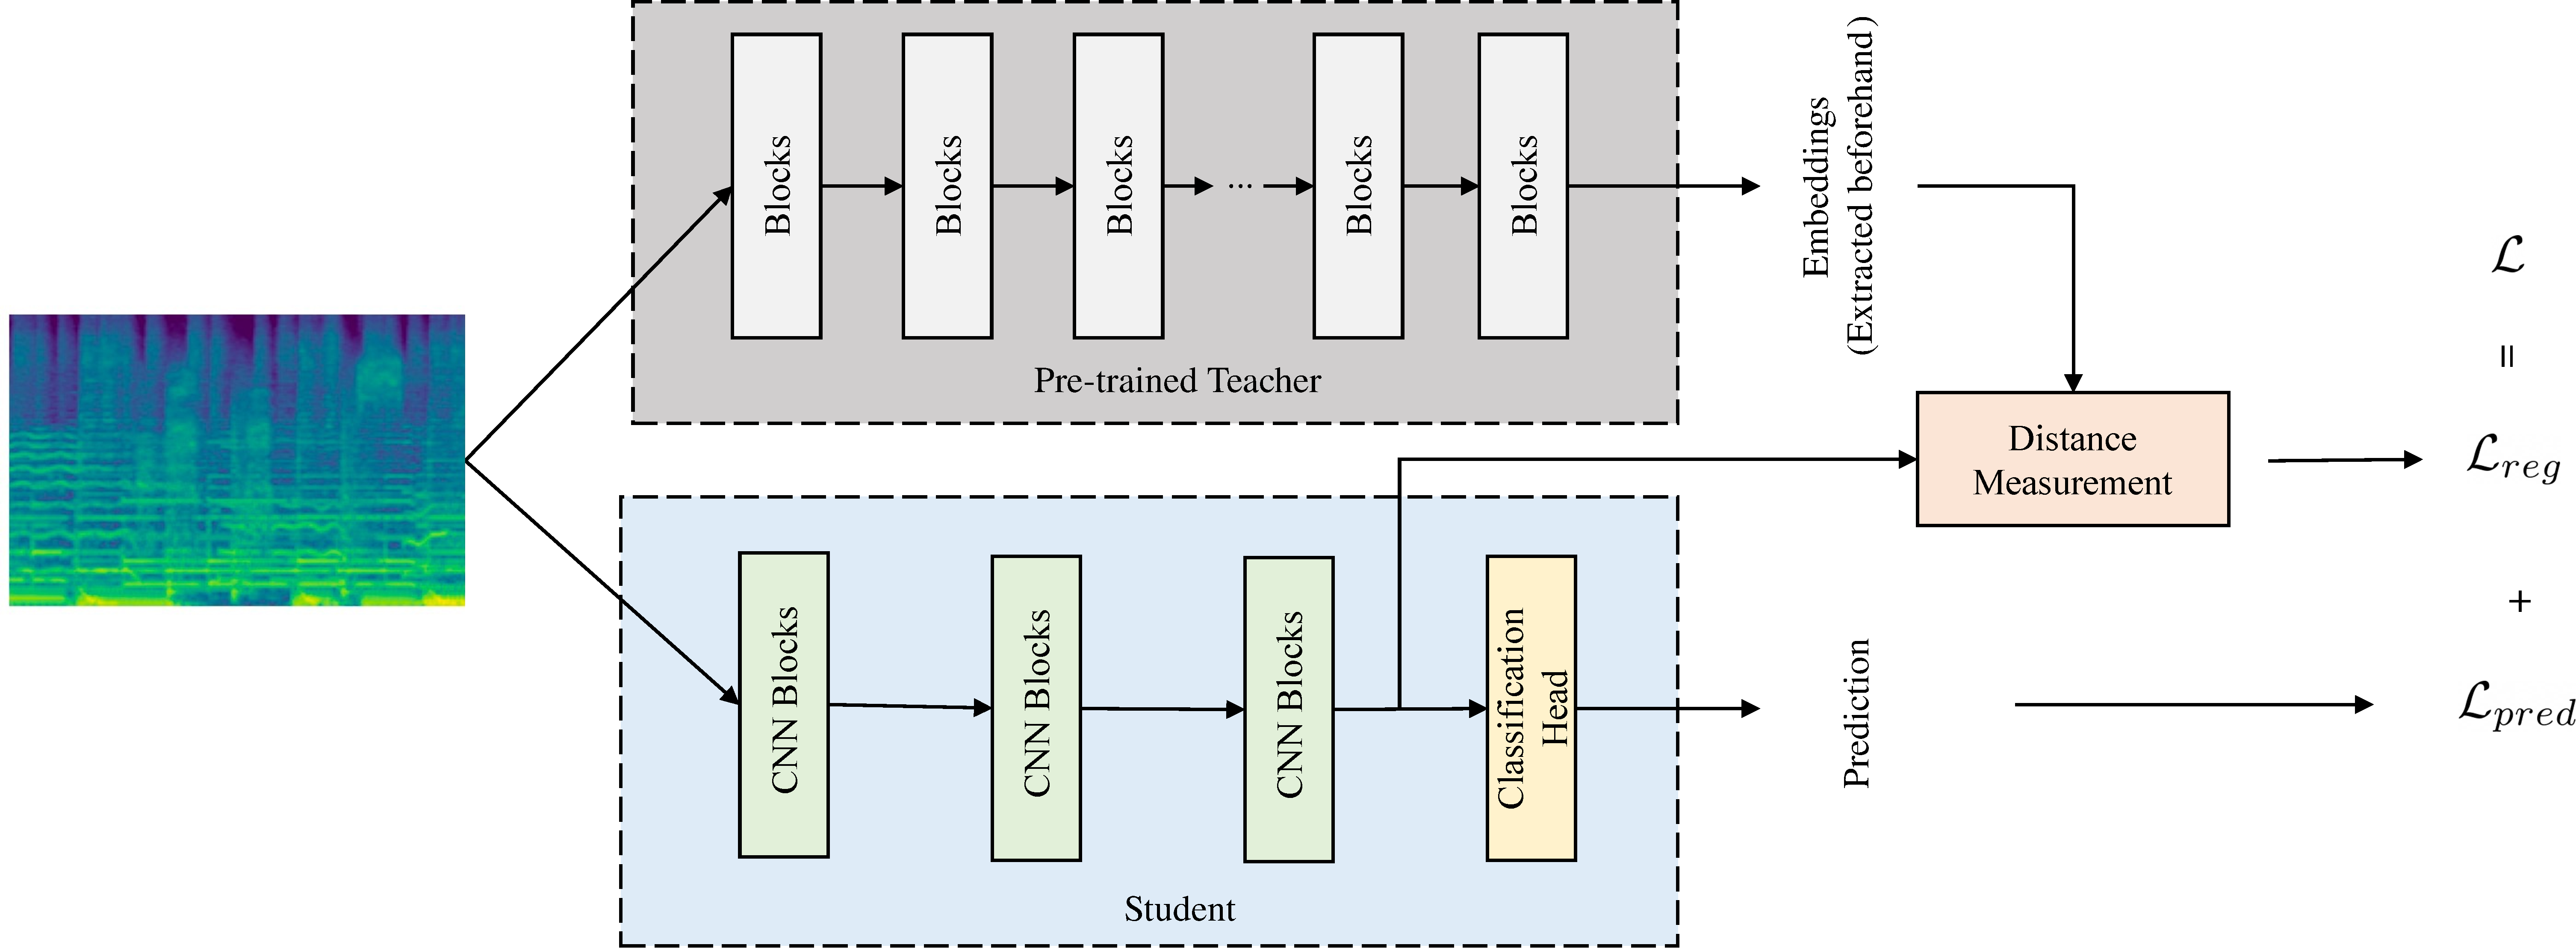
\includegraphics[width=.8\linewidth]{east-pipeline}%
    \end{figure}
    \bigskip
    \begin{itemize}
        \item   \textbf{transfer learning}
            \begin{itemize}
                \item   use embeddings from a different task for the target task
            \end{itemize}
            \smallskip
        \item   \textbf{knowledge distillation}
            \begin{itemize}
                \item   use a teacher to train a less complex student on the same task
            \end{itemize}
    \end{itemize}
\end{frame}

\begin{frame}{embeddings as teachers}{experimental setup}
            \begin{itemize}
                \item   task: auto-tagging
                    \begin{itemize}
                       \item   MagnaTagATune (MTAT) dataset:
													\begin{itemize}
															\item   50 music tags
															\item   \unit[30]{s} audio snippets ($\approx$ 21000)
													\end{itemize}
                    \end{itemize}
                \bigskip
                \item   systems:
                    \begin{itemize}
                        \item   baseline: student without teacher
                        \item   teacher: embedding plus logistic regression
														\begin{itemize}
															\item VGGish
															\item OpenL3
															\item PaSST
															\item PANNs
														\end{itemize}
												\item		KD: student trained with soft targets from teacher
												\item		EAsT: student regularized with teacher embeddings
                    \end{itemize}
            \end{itemize}
\end{frame}

%\begin{frame}{embeddings as teachers}{experimental setup: data}
    %\begin{columns}
        %\column{.8\linewidth}
            %\begin{itemize}
                %\item   DCASE 17:
                    %\begin{itemize}
                        %\item   17 audio event classes
                        %\item   \unit[10]{s} audio snippets ($\approx$ 53000)
                    %\end{itemize}
                %\bigskip
                %\item   MagnaTagATune (MTAT):
                    %\begin{itemize}
                        %\item   50 music tags
                        %\item   \unit[30]{s} audio snippets ($\approx$ 21000)
                    %\end{itemize}
            %\end{itemize}
        %\column{.2\linewidth}
    %\end{columns}
%\end{frame}

\begin{frame}{embeddings as teachers}{results}
    \vspace{-3mm}
    %\begin{footnotesize}
%\begin{table}
    %\begin{center}
    %\begin{tabular*}{\textwidth}{l|@{\extracolsep{\fill}}cccccccccc}
    %%\begin{tabular}{lcccccccccc}
        %% \hlineB{4}
        %\hline
        %\hline
        %
        %% \multicolumn{11}{c}{OpenMIC}\\
        %
        %% \hlineB{4}
        %% \hline
        %%Feature
        %\multirow{2}{*}{\textbf{OpenMIC}}
                %& \multicolumn{2}{c}{None}
                %& \multicolumn{2}{c}{VGGish}   & \multicolumn{2}{c}{OpenL3}
                %& \multicolumn{2}{c}{PaSST}    & \multicolumn{2}{c}{PANNs}\\
        %\cline{2-11}
        %%Models
                %& mAP           & F1
                %& mAP           & F1            & mAP           & F1
                %& mAP           & F1            & mAP           & F1\\
        %\hline
        %%CP ResNet* \cite{koutini2021receptive}  & .819          & .809
                %%& -     & -     & -     & -     & -     & -     & -     & -\\
        %SS CP ResNet %\cite{koutini2021receptive}  
								%& .831          & .822   & -     & -     & -     & -     & -     & -     & -     & -\\
        %\hline
        %Teacher\textsubscript{LR} & - & -
                %& .803          & .799          & .803          & .798
                %& \textbf{.858} & \textbf{.837} & \textbf{.853}          &\textbf{.834}\\
        %% KD (w/o mask) ** 
        %%         & .839          & .825          & .827          & .816
        %%         & .853          & .837          & .854          & .832\\
        %KD (w/ mask) & - & -
                %& .829          & .820          & .823          & .813
                %& .851          & {.834}          & .848          & .823\\
        %\hline
        %%EAsT\textsubscript{Cos-Diff} & - & -
                %%& .838          & .824          & {\textbf{.838}} & .820
                %%& .837          & .822          & .836          & .814\\
        %EAsT\textsubscript{Final} & - & -
                %& {\textbf{.842}}     & {\textbf{.828}} 
                %& \textbf{.835}          & {\textbf{.822}}
                %& .847          & .830          & .849          & .828\\
        %% Global + Last Stage
        %%         & .835          & .821          & .830          & \textbf{.823}
        %%         & .842          & .826          & .839          & .823\\
        %%EAsT\textsubscript{All} & - & -
                %%& .836          & .823          & .835          & {\textbf{.822}}
                %%& .845          & .827          & .845          & .827\\
        %% Global + All stages
        %%         & .836          & .820          & .829          & .816
        %%         & .839          & .825          & .841          & \textbf{.831}\\
        %%EAsT\textsubscript{KD} & - & -
                %%& .836          & .825          & .836          & .821
                %%& {.852}              & {.834}       
                %%& {\textbf{.857}}     & {.831}\\
        %% \hlineB{4}
        %\hline
        %\hline
%
        %\\
%
        %% \hlineB{4}
        %\hline
        %\hline
        %%Feature 
        %\multirow{2}{*}{\textbf{MagnaTagATune}}
                %& \multicolumn{2}{c}{None}
                %& \multicolumn{2}{c}{VGGish}   & \multicolumn{2}{c}{OpenL3}
                %& \multicolumn{2}{c}{PaSST}    & \multicolumn{2}{c}{PANNs}\\
        %\cline{2-11}
        %%Models
                %& mAP           & AUC
                %& mAP           & AUC            & mAP           & AUC
                %& mAP           & AUC            & mAP           & AUC\\
        %\hline
        %%FCN$^\dagger$    \cite{choi2016automatic}   & .429          & .900
                %%& -     & -     & -     & -     & -     & -     & -     & -\\
        %Mobile FCN 
                %& .437          & .905
                %& -     & -     & -     & -     & -     & -     & -     & -\\
        %% \yiwei{SOTA}    \cite{choi2016automatic}   & .461          & .913
        %%         & -     & -     & -     & -     & -     & -     & -     & -\\
        %\hline
        %Teacher\textsubscript{LR} & -             & -
                %& .433          & .903          & .403          & .890
                %& \textbf{.473} & \textbf{.917} & \textbf{.460} & \textbf{.911}\\
        %KD      & -             & -
                %& .447          & .911          & .439          & .907
                %& .454          & .912          & .448          & .909\\
        %\hline
        %%EAsT\textsubscript{Cos-Diff} & -             & -
                %%& .446          & .906          & .438          & .907
                %%& .453          & .912          & .453          & .911\\
        %EAsT\textsubscript{Final}
                %& -             & -
                %& \textbf{.454}          & {\textbf{.912}} & \textbf{.447}          & \textbf{ 	}
                %& .459          & .912          & .449          & .909\\
        %% Global + Last Stage
        %%         & .448          & .910          & .437          & .905
        %%         & .456          & .914          & .452          & .910\\
        %%EAsT\textsubscript{All}
                %%& -             & -
                %%& {\textbf{.455}}     & .911          
                %%& {\textbf{.452}}     & {\textbf{.911}}
                %%& .458          & .913          & .457          & .911\\
        %% Global + All Stages
        %%         & .438          & .905          & .433          & .902
        %%         & .449          & .909          & \textbf{.463} & \textbf{.912}\\
        %%EAsT\textsubscript{KD}
                %%& -             & -
                %%& .441          & .908          & .437          & .904
                %%& {.461}              & {.915}          
                %%& {.459}              & {\textbf{.912}}\\
        %% \hlineB{4}
        %\hline
        %\hline
    %\end{tabular*}
    %\end{center}
    %\label{tab:east-results}
    %%\vspace{-1mm}
%\end{table}
    %\end{footnotesize}
    
    \begin{columns}
			\column{.6\linewidth}
			\begin{itemize}
					\item   student model consistently outperforms baseline
					\smallskip
					\item   student model consistently outperforms knowledge distillation
					\smallskip
					\item   student model outperforms teacher for "old" embeddings
					\smallskip
					\item   modern embeddings are powerful but complex
			\end{itemize}
    \column{.4\linewidth}
			\begin{figure}
			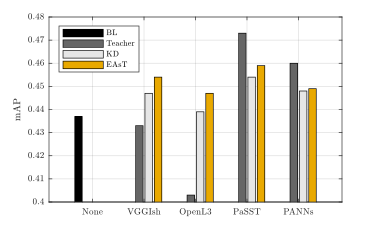
\includegraphics[width=1.15\columnwidth]{east-results}
			\end{figure}
		\end{columns}
		\phantom{\footfullcite{ding_audio_2023}}
\end{frame}

%\begin{frame}{embeddings as teachers}{results: data dependency}
    %\begin{itemize}
        %\item   Con-Reg outperforms non-regularized system in all cases
        %\item   larger improvement for lower amounts of data
    %\end{itemize}
    %\begin{figure}%
        %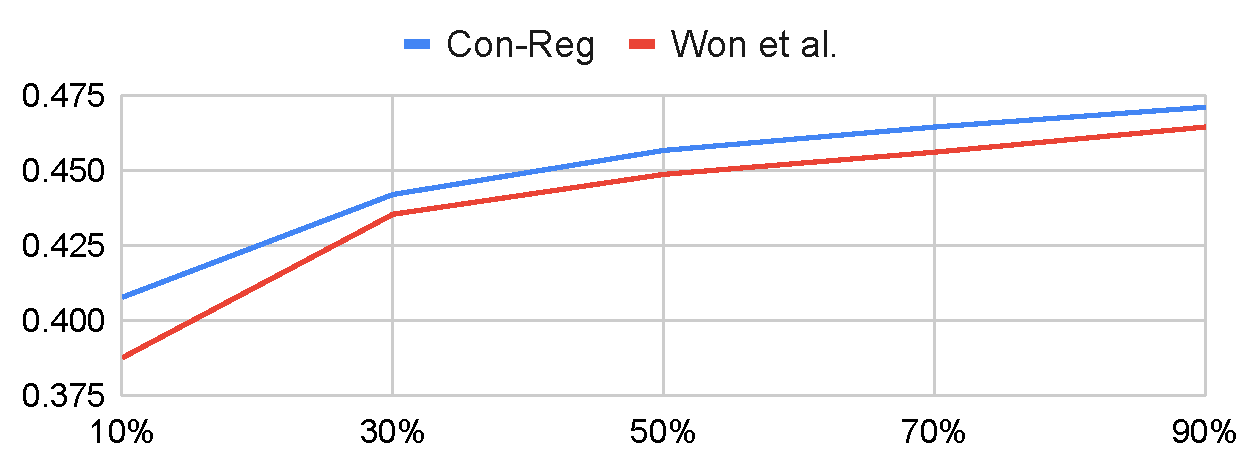
\includegraphics[scale=.45]{rep-results-data}
    %\end{figure}
    %
    %\phantom{\footfullcite{hung_feature-informed_2022}}
%\end{frame}
 